\section{Probenpräparation}
Für die Probenpräparation einer Silizium Probe für eine TEM Messung müssen viele einzelne schritte durchlaufen werden.
Zu Beginn wird ein Silizium Wafer verwendet, dieser hat ein Durchmesser von ca. 15 cm und eine Stärke von ca. 700µm. Durch Anritzen einlag der Kristallstruktur mit einer Diamant Ahle und durch Zuhilfenahme einer Brechzange kann der Wafer in eine handliche Größe gebrochen werden.
Zwei Wafer Stücke in passender Größe und Kristall Orientierung werden mit einem G1 Epoxid Kleber wie ein Sandwich aneinandergeklebt. Dieses Wafer Sandwich kann nun durch Zuhilfenahme einer Diamant Fadensäge in eine gewünschte Größe geschnitten werden (1,5x1,5x30mm).

\begin{figure}[htbp]
 \centering
 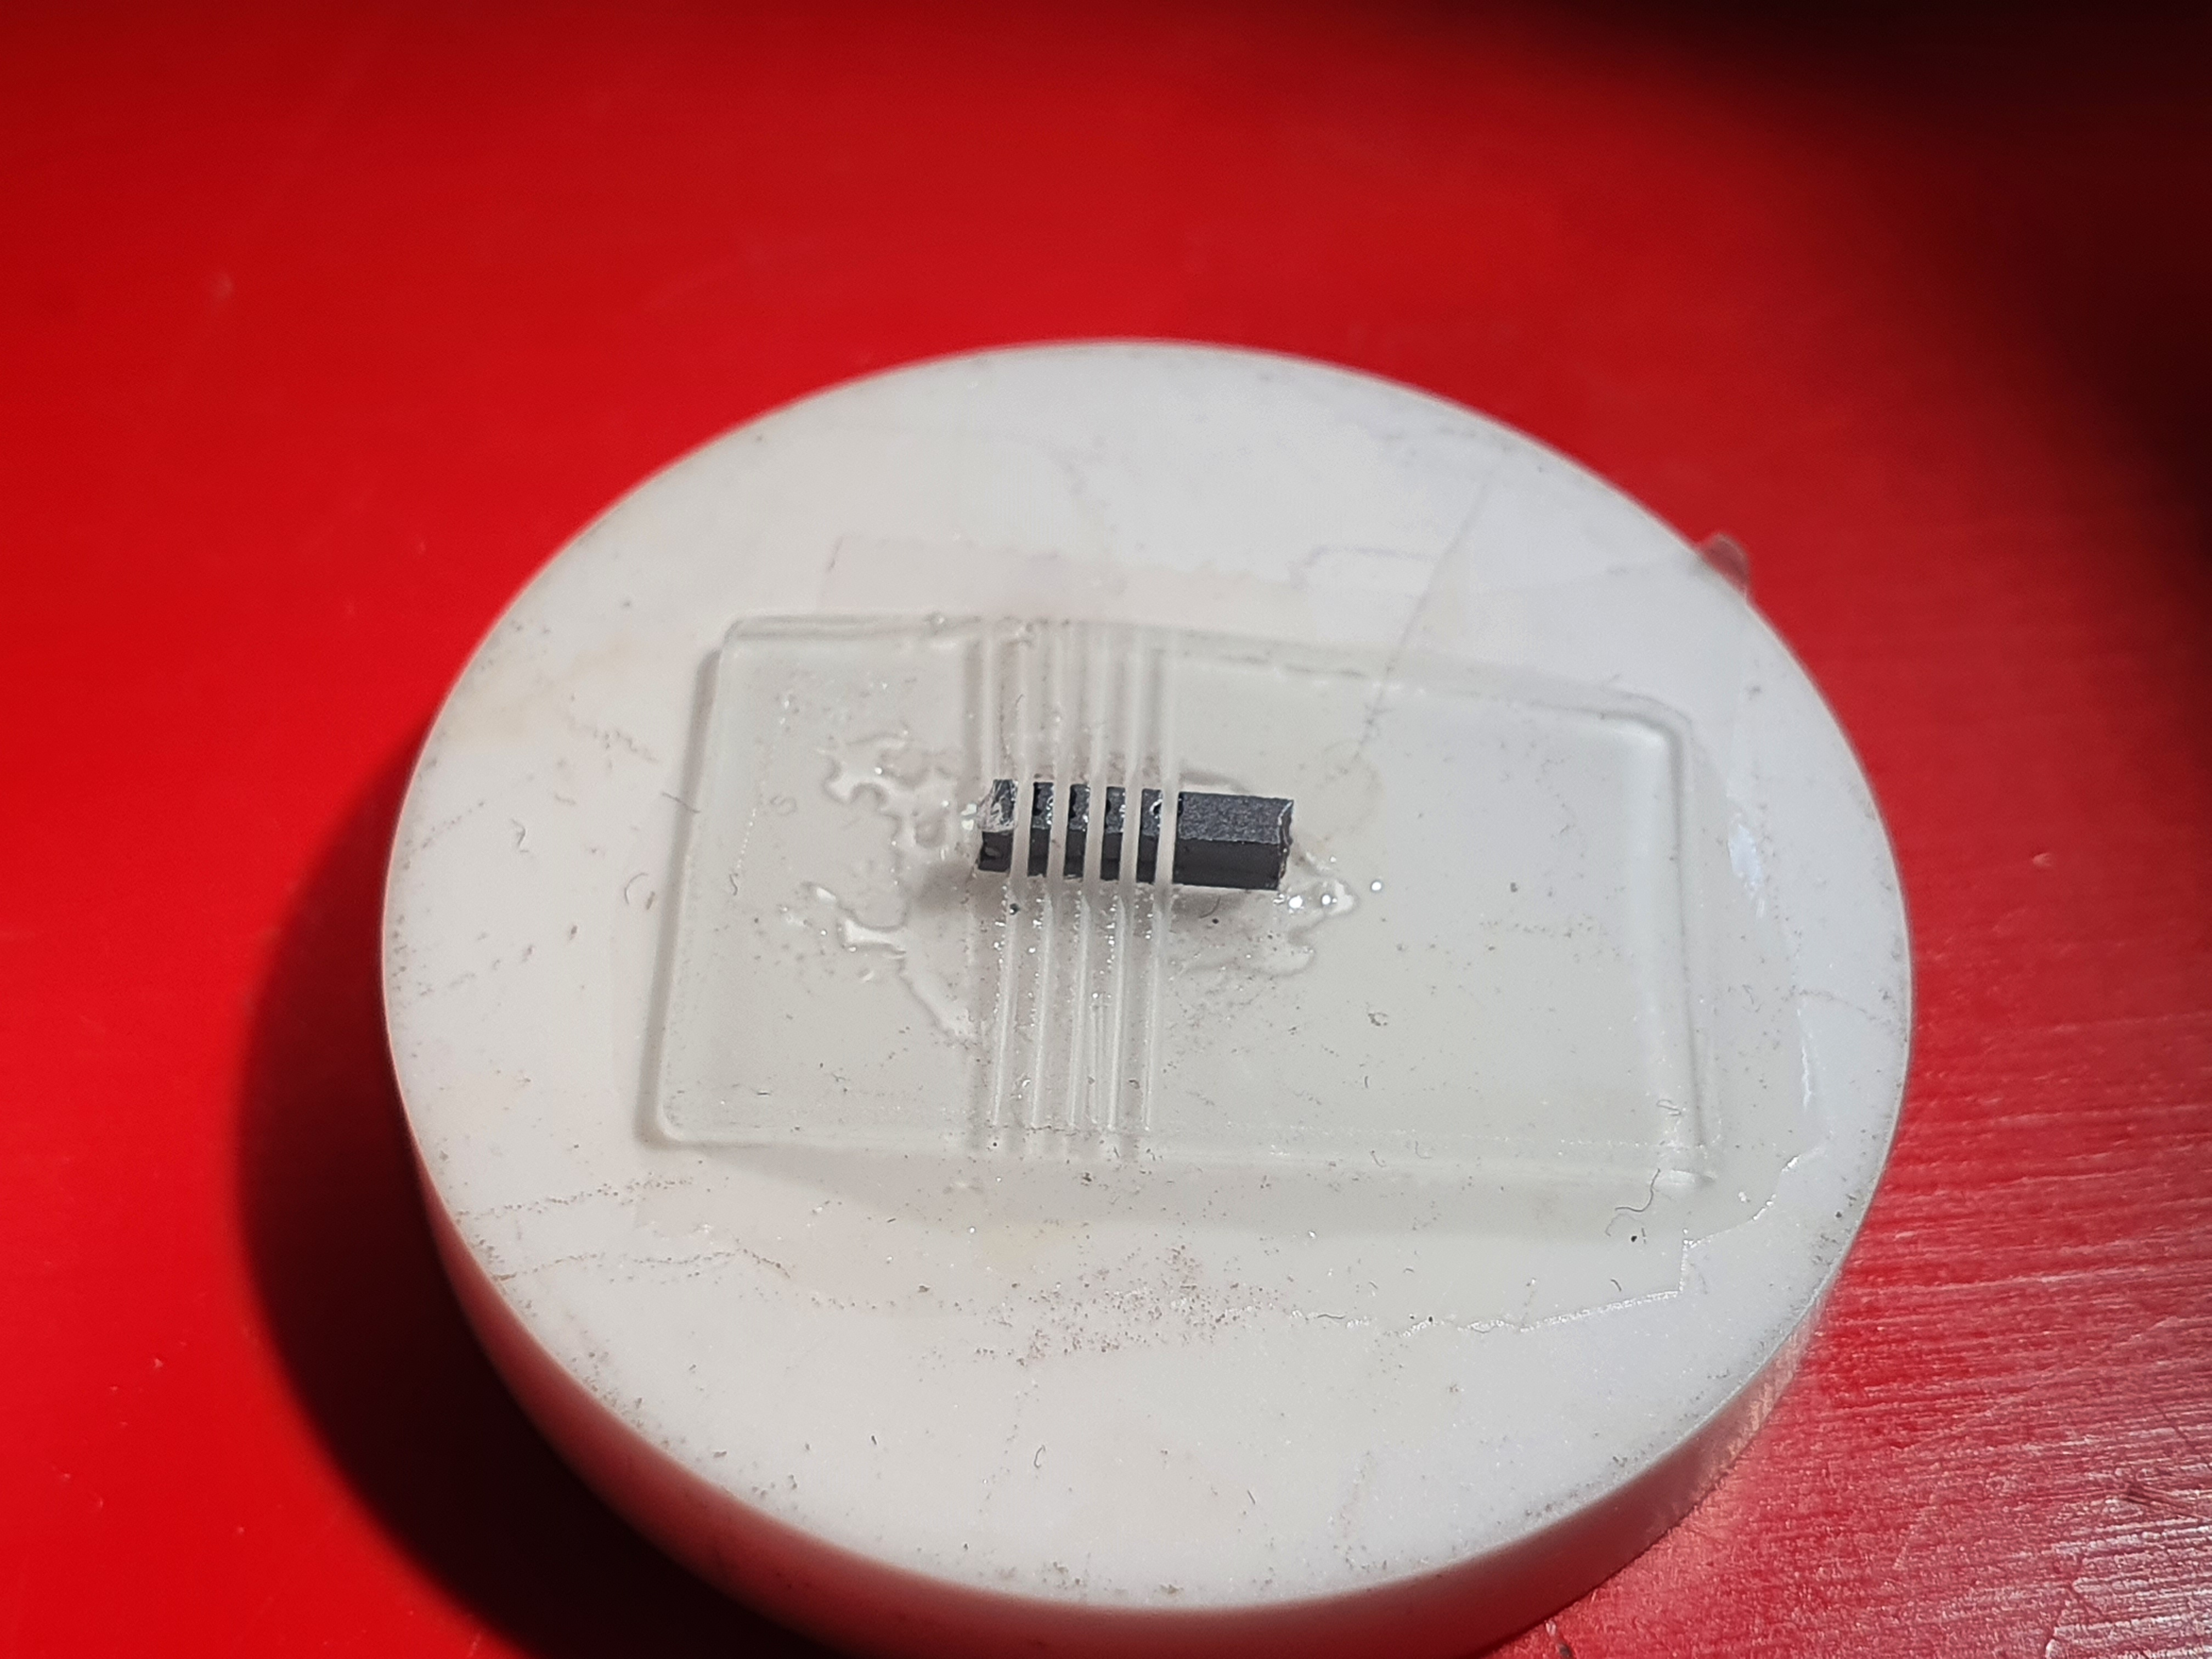
\includegraphics[width=0.7\textwidth]{Gerüst/Abbildungen/Proben/20220607_101331.jpg}
 \caption[Si Sandwich]{Si Sandwich mit Diamant Säge in Segmente geschnitten, Auf Glas Träger aufgeklebt.}
 \label{DiamantSege}
\end{figure}

Das Wafer Sandwich wird dann unter dem optischen Mikroskop auf eine gleichmäßige Kleberschichtdicke und mögliche Defekte in der Probe untersucht. Wenn die Probe zufriedenstellend ist, kann das Sandwisch nun mit der Fadensäge ich feine Streifen geschnitten werden. Dies erfolgt senkrecht zur Verklebung Achse, um die klebe Schicht anschließen in der Mitte der abgeschnittenen Proben Plättchen zu erhalten. Die geplante Schichtdicke der abgeschnitten scheiben wird auf 400 µm am Gerät eingestellt. Beim Abschneiden ist der auf eine gute Befestigung am probenträger durch Ankleben, eine passende Fadenspannung, anpressdruck den Schneidfaden und eine ausreichende Kühlung durch Wasser zu achten. Es wurden 5 scheiben aus dem Sandwich herausgeschnitten um bei potenziellem Bruch der Scheiben ausreichend Reserve zu ermöglichen.
Eine gut intakte Schreibe, die dem erwarteten dicken endspricht, wurde unter dem Optischen Mikroskop auf einen Titan Probenhalterring montiert. Hierfür wurde zunächst der Titanring erst leicht verbogen, um die Probe mechanisch an den Probenhalter zu fixieren. Anschließen wurde die Probe mit dem G1 Epoxid Kleber am Probenhalter verklebt. Dabei musste unter dem optischen Mikroskop darauf geachtet werden das keine Luft Einschlüsse endstehen. Nach Aushärtung des Klebers auf einer Wärmeplatte bei 130°C sind Klebers und Silikon überstände entfernt worden. Dafür wurde eine 1000 Körnung Siliciumcarbid Schleifscheibe verwendet zusammen mit einem Skalpell unter dem Optischen Mikroskop. Es musste darauf geachtet werden das gleichmäßig geschleiften wird bis das Titan des Probenhalter gleichmäßig am gesamten ring reflektiert. Beide Seiten wurden so bearbeitet so das eine gesamte Probendicke von ca. 300 µm entstand, dies ist die dicke des Titan Probenhalterring.

\begin{figure}[htbp]
 \centering
 \includegraphics[width=0.7\textwidth]{Gerüst/Abbildungen/Proben/20220607_104115.jpg}
 \caption[Probenhalter]{Probe im Titan Probe Halter ein geklemmt, noch nicht verklebt.}
 \label{Probenhalter}
\end{figure}

Am Optischen Mikroskop ist erneut überprüft worden, ob das Abtragen des überstand, gelungen ist und ob die Probe irgendwelche defekte aufwies.
Die probendicke ist nun mit Hilfe eines digitalen Dickenmesser auf einer Granitplatte ausgemessen worden und eine durchschnittlichen dicke von 308,4µm wurde gemessen.
Die Probe wurde nun auf einen Glasträger mit einem Temperaturlöslichen Klebers befestigt.
Mit Hilfe eines Diskgrinder der eine akkurate abtragungstiefe und Parallelität gewährleistet wurde die Probe plan abgeschliffen, dabei ist eine Dimant Schleifpaste mit einer 3µm Korn Größe zum Einsatz gekommen.  
Mit einem Dickenmesser wurde nun die dicke des Glasträgers (9379,4µm), der Probe (308,4µm) und der Klebeschicht (1,9µm) gemessen. Dabei ist auf die Orientierung der Probe geachtet worden, um wiederholbare Messungen durführen zu können. Die Proben werden beim Messen immer an allen vier Seiten des Titan Rings gemessen und gemittelt, um spätere dicken Bestimmungen nach dem Dimplen nachvollziehbar zu ermöglichen.
Auf der Ersten Seite wurde nun ein Dimple (Mulde) eingeschliffen, hierfür ist ein Dimpler zu Einsatz gekommen. Der Dimple schneidet eine Mulde mit Hilfe eines Schleif Rad und eines sich drehenden Werkstückhalter.

Die ersten Arbeitsschritte ist die Zentrierung der Probe auf dem Werkstückhalter, dabei wird versucht das Rotationszentrum auf gleich mit dem klebe Schicht in der Probe zu bringen und die Tiefeneichung der Schleifscheibe einzustellen. 
Zuerst wurde die Probe mit einer Bronze Rad in Kombination mit einer 3µm Dimant Schleifpaste bearbeitet. Es wurde eine geplante Dimpel tief von 35µm im Dimpler eingestellt und ausgeführt.
Nach dem Reinigen der Probe ist mithilfe eines optischen Mikroskops die erzeugte Dimlpetiefe gemessen worden. Dabei wird das Mikroskop zuerst am proben Rand fokussiert und dann am Dimpel Zentrum, der Probentischhöhen Unterschied zwischen diesen Messungen ist die Dimpletiefe. Nach der ersten Abtragungsstritt wurde eine tiefe von 33µm gemessen.
Beim Zweiten Abtragungsstritt wird der Dimpel mit einem Filz Rad und einer Diamant Politurpaste von 1µm bearbeitet. Dabei wird die Probe für 5 Minuten bearbeite.
Bei der anschließenden tiefen Bestimmung durch das optische Mikroskop konnte eine tiefe von 37µm festgestellt werden. 
Im letzten Abtragungsstritt wurde ein Filz Rad mit einer Diamant Politur mit einer Körnung von 0,25µm verwendet. Hierbei wurde wieder 5 Minuten poliert.
Das optische Mikroskop hat wieder eine Dimpeltiefe von 37 µm bestimmt, zudem konnte die Oberfläche der Probe unter die Mikroskope auf übergebliebene schleif Kratzers und defekte untersucht werden.

\begin{figure}[htbp]
 \centering
 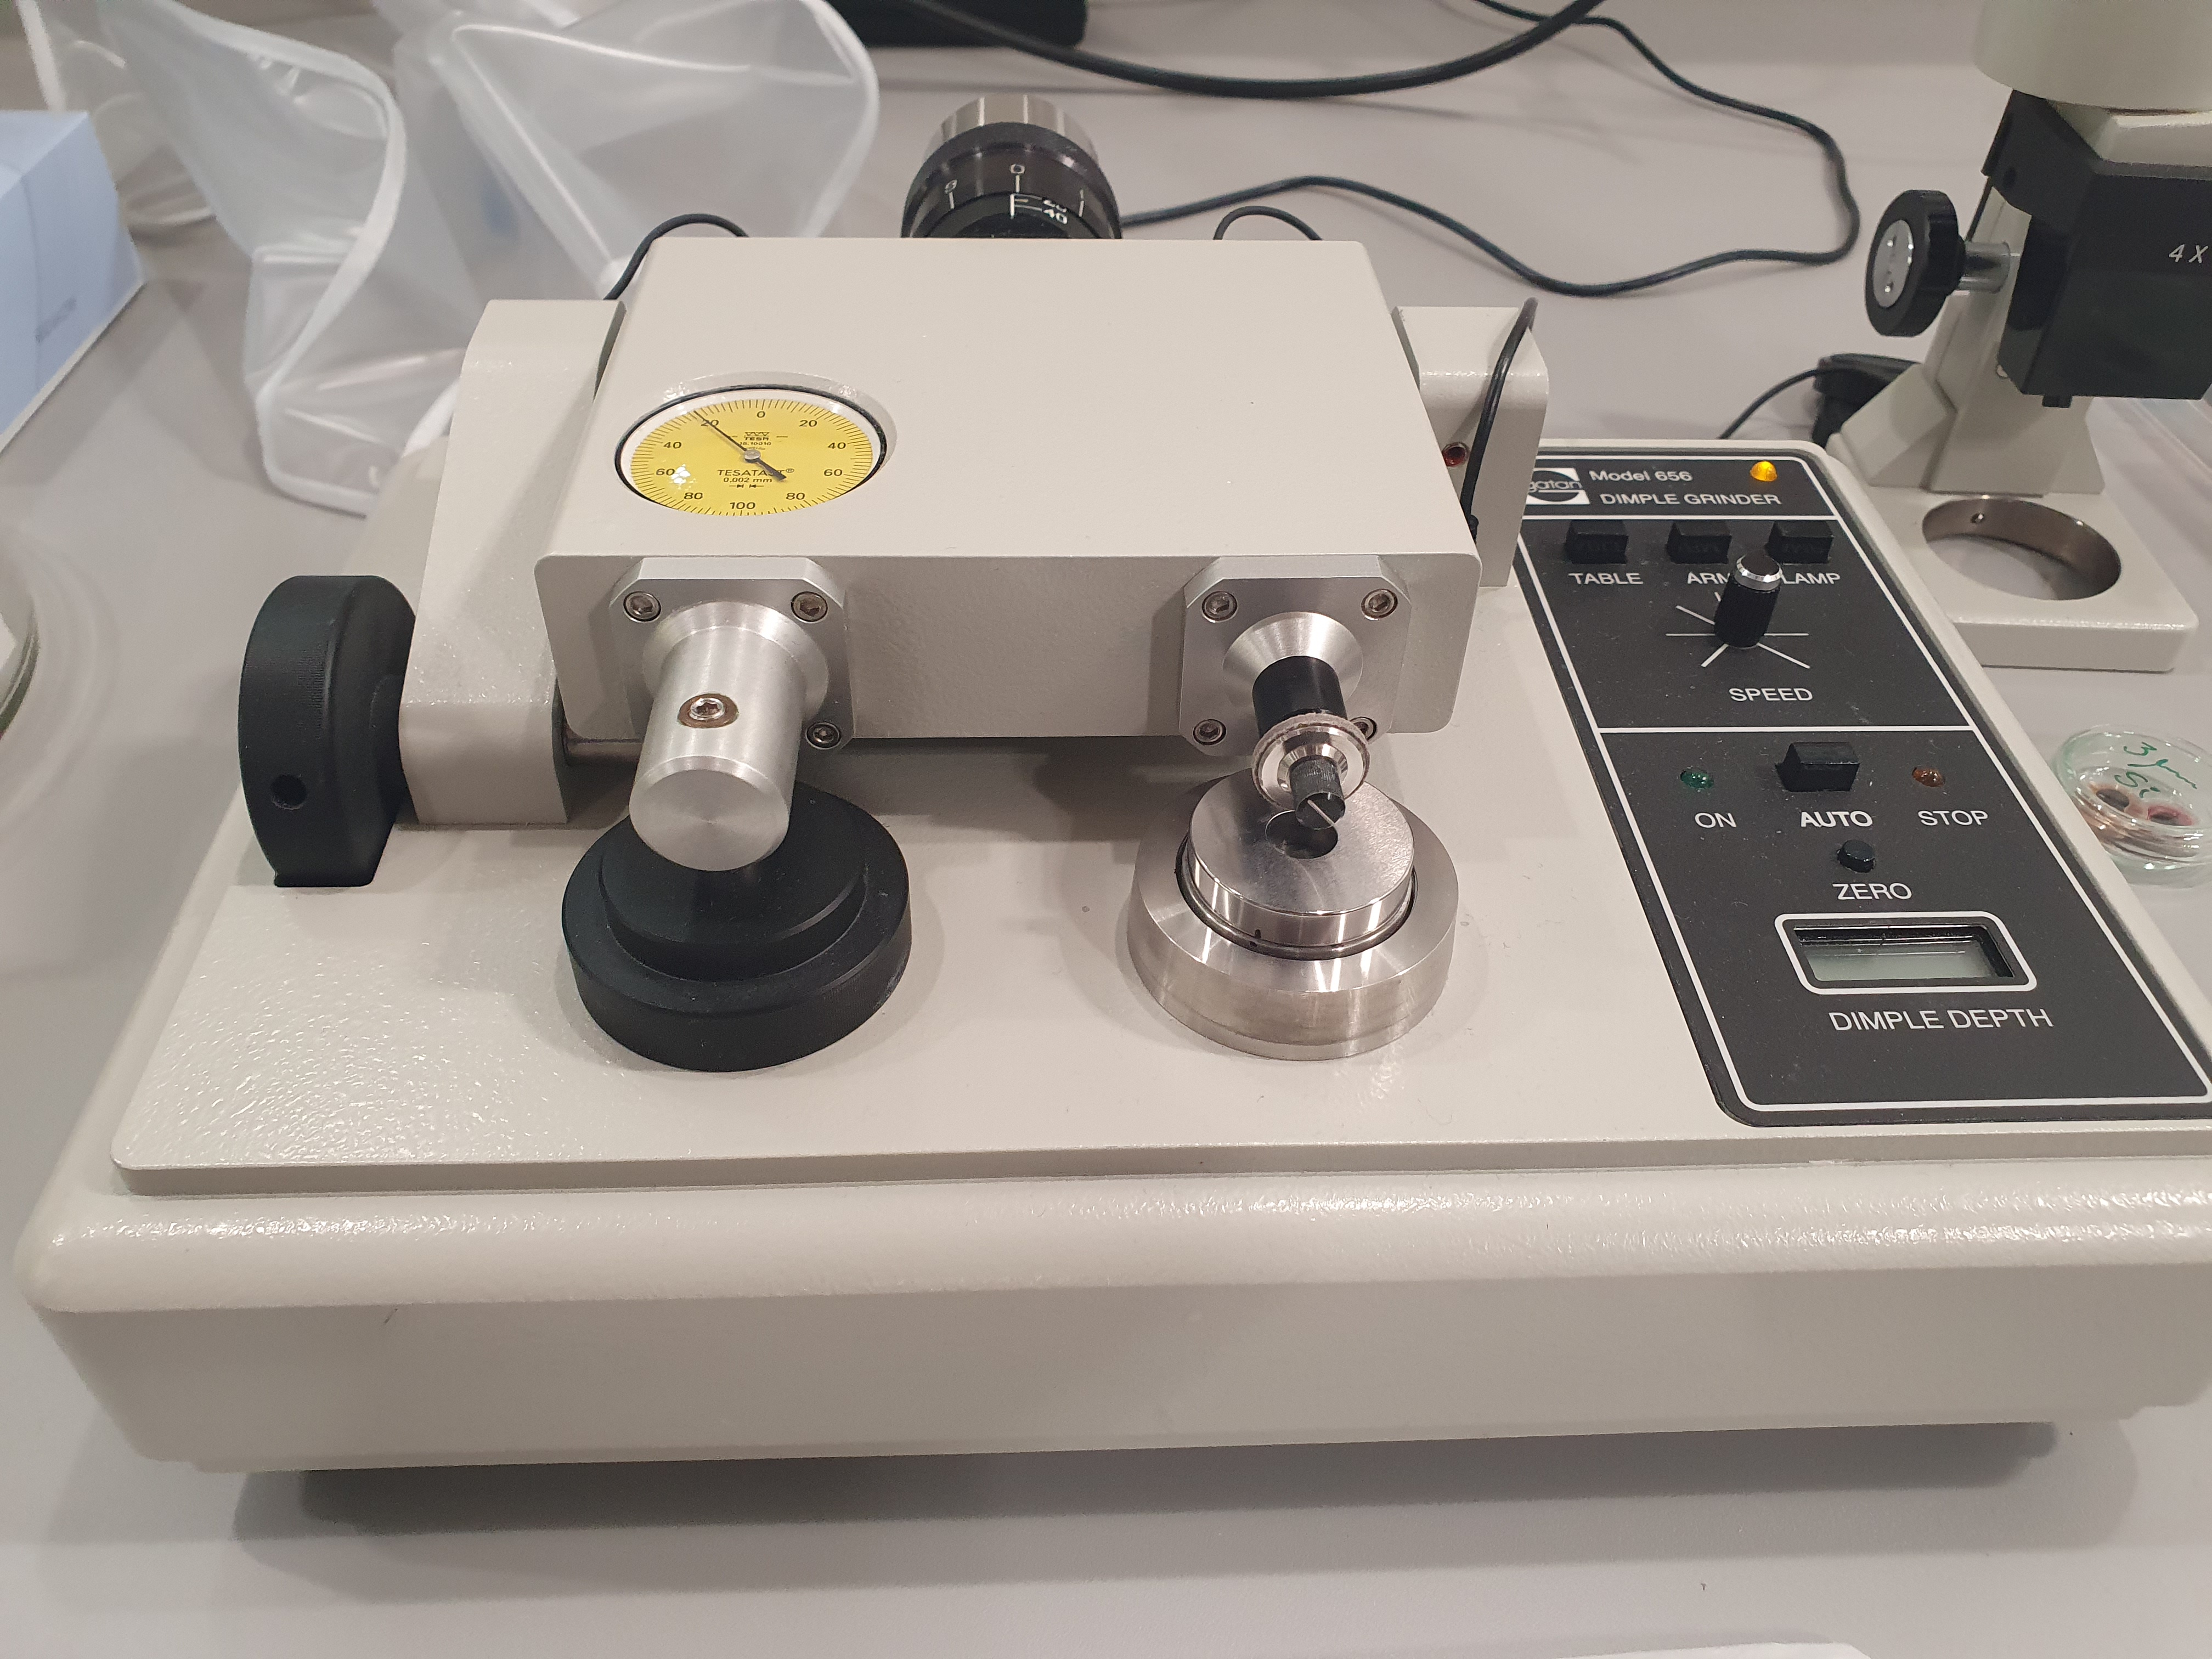
\includegraphics[width=0.7\textwidth]{Gerüst/Abbildungen/Proben/20220607_144532.jpg}
 \caption[Dimpler]{Dimpler mit Filz Polierscheibe.}
 \label{Dimpler}
\end{figure}

Die Probe wurde nun durch Erhitzen an der Wärme platte und ausflössen der Kleber im Azeton Bad von Glasträger gelöst werden. Anschließen wurde die Probe mit der gedimpleten Seite nach unten wieder auf dem Glas Träger geklebt. Dabei ist die Orientierung der Maskierung auf der Probe berücksichtigt worden.

Die Schichtdicke des Klebers wurde wieder am Dickenmesser gemessen um einerseits eine geringe klebe schickt du garantieren und andererseits, um die Parallelität zur bereits Seiten der Probe zu gewährleisten.
Anschließend wurde die gewünschte Probendicke am Zentrum der Probe Bestimmt welch nach dem dimplen der zweiten Seite 10µm betragen sollte. Um dies zu erreichen wurde beschlossen die gesamt proben dicke auf 80µm zu verdünnen und eine Dimpletiefe von 20 µm einzuschleifen.
Mit dem Diskgrinder und der 3µm Diamant Schleifpaste wurde bei der gesamten Probe 120µm abgetragen so das nach dem messenden auf den Dickenmesser eine gemittelte probendicke von 78,75µm festgestellt wurde. 

Das Diplen wurde wie auf der ersten Seite durchgeführt. Nach dem ersten Ausdünnunen mit dem Bronzerad und 3µm Schleifpaste wurde eine Dimpeltiefe von 19,5 µm am optischen Mikroskop festgestellt. Nach der ersten Politur bei 1µm von 7 Minuten und der Zweiten Politur bei 0,25µm und 10minuten konnte eine klares durchscheinen durch die Probe auf dem Dimpler festgestellt werden.
Am Optischen Mikroskop konnte dann eine Dimpeltiefe von 27µm gemessen werden. Es wurden keine defekte, Risse oder andere Verunreinigungen am Mikroskop in der Probe gefunden, und eine gute Kristallstruktur war an der polierten Oberfläche erkennbar.
Die Probe wurde anschließend im Azeton Bad vom Glasträger gelöst und gereinigt.

\begin{figure}[htbp]
 \centering
 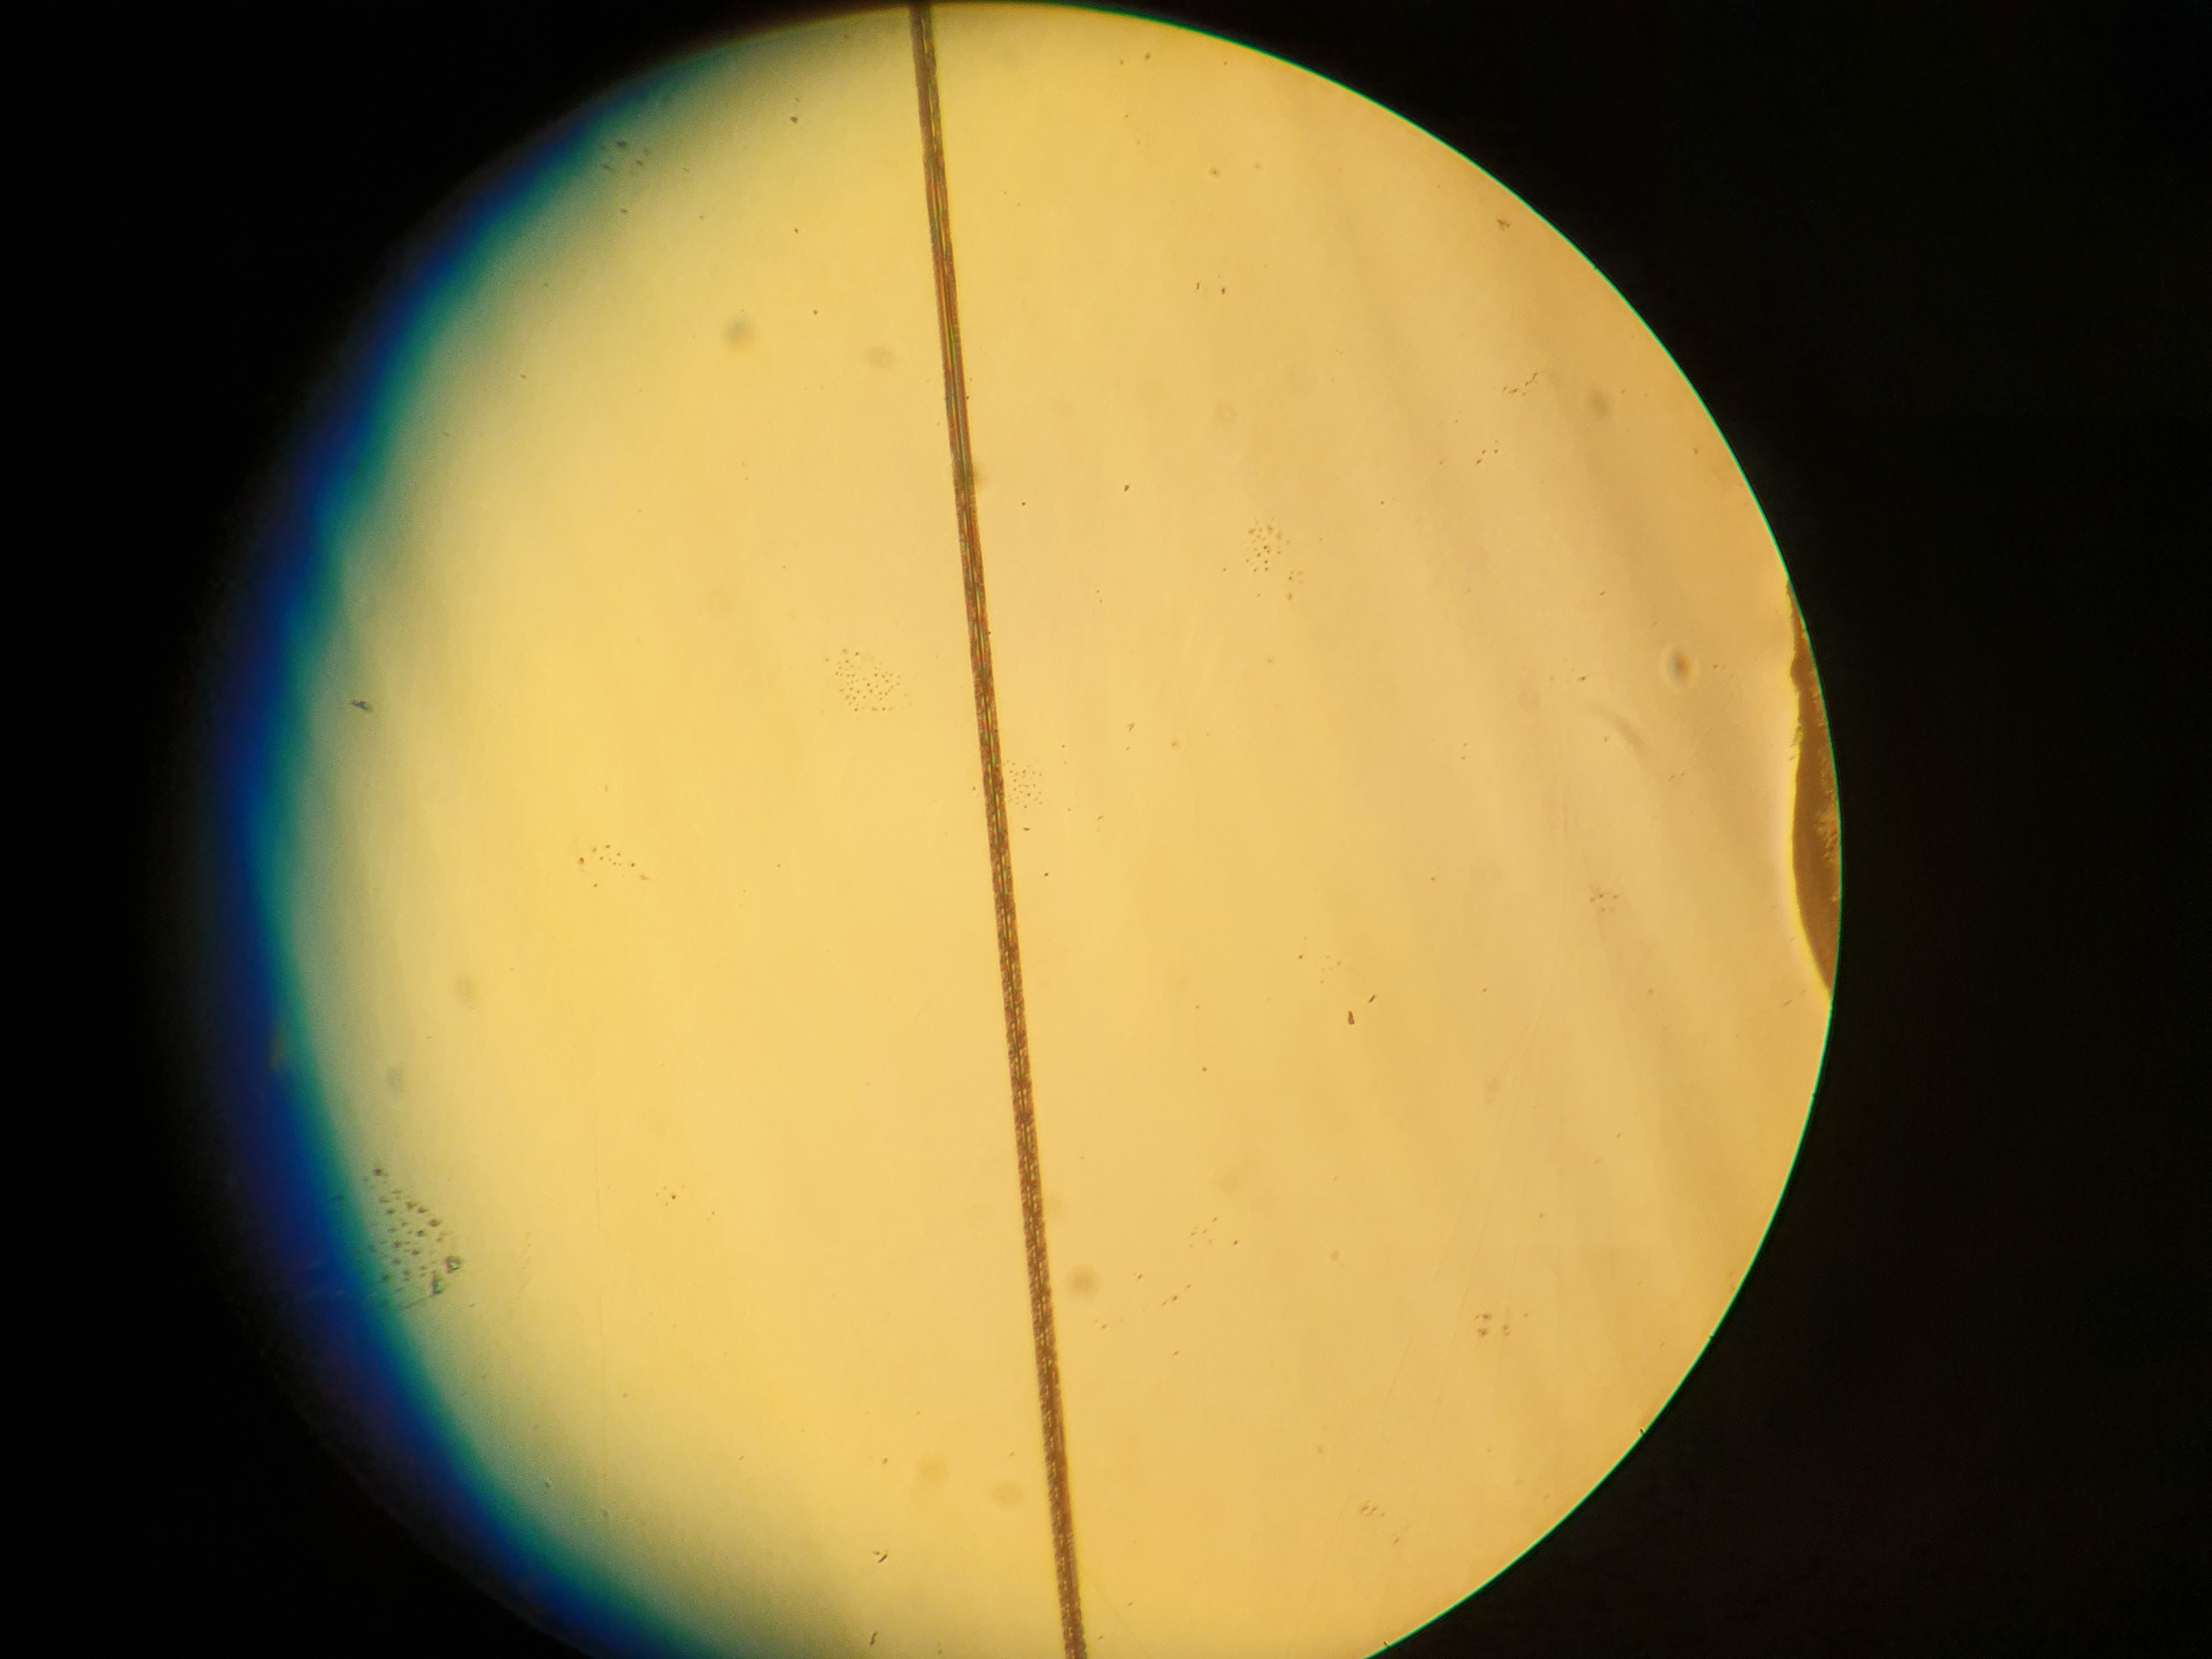
\includegraphics[width=0.7\textwidth]{Gerüst/Abbildungen/Proben/20220609_104730.jpg}
 \caption[OptMikro]{Klebeschicht zwischen dem Si Wafer im Optischen Mikroskop, es ist eine leicht Kristall Struktur erkennbar.}
 \label{OptMikro}
\end{figure}

Die Ionen Dünnung konnte aus Zeitlichen Gründen nicht mehr durchgeführt werden, dies wurde jedoch von Silke Stöwer abgeschlossen. Es wurde die Handhabung und einbaut der Probe in die Ionen Dünnung demonstriert und diskutiert. Jedoch sind uns keine Messergebnisse der Ionen Dünnung bekannt.
